\chapter{Egyenletek}
\label{sec:Egyenletek}

\section{Kvantum séta a rácson}

A következőkben a rácson, mint 4-reguláris gráfon vett bolyongást fogjuk
részletesen megvizsgálni.

Legyen a rács $N = n \times n$ -es.


\begin{figure}[!ht]
  \begin{center}
    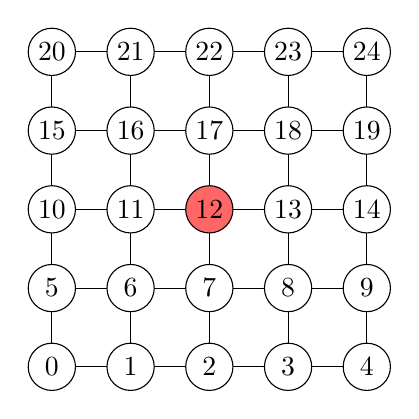
\begin{tikzpicture}

      \draw(0,0) -- (0,4);
      \draw(1,0) -- (1,4);
      \draw(2,0) -- (2,4);
      \draw(3,0) -- (3,4);
      \draw(4,0) -- (4,4);

      \draw(0,0) -- (4,0);
      \draw(0,1) -- (4,1);
      \draw(0,2) -- (4,2);
      \draw(0,3) -- (4,3);
      \draw(0,4) -- (4,4);

      \draw[black,fill=white](0,0) circle (0.3) node {0};
      \draw[black,fill=white](1,0) circle (0.3) node {1};
      \draw[black,fill=white](2,0) circle (0.3) node {2};
      \draw[black,fill=white](3,0) circle (0.3) node {3};
      \draw[black,fill=white](4,0) circle (0.3) node {4};

      \draw[black,fill=white](0,1) circle (0.3) node {5};
      \draw[black,fill=white](1,1) circle (0.3) node {6};
      \draw[black,fill=white](2,1) circle (0.3) node {7};
      \draw[black,fill=white](3,1) circle (0.3) node {8};
      \draw[black,fill=white](4,1) circle (0.3) node {9};

      \draw[black,fill=white](0,2) circle (0.3) node {10};
      \draw[black,fill=white](1,2) circle (0.3) node {11};
      \draw[black,fill=red!60](2,2) circle (0.3) node {12};
      \draw[black,fill=white](3,2) circle (0.3) node {13};
      \draw[black,fill=white](4,2) circle (0.3) node {14};

      \draw[black,fill=white](0,3) circle (0.3) node {15};
      \draw[black,fill=white](1,3) circle (0.3) node {16};
      \draw[black,fill=white](2,3) circle (0.3) node {17};
      \draw[black,fill=white](3,3) circle (0.3) node {18};
      \draw[black,fill=white](4,3) circle (0.3) node {19};

      \draw[black,fill=white](0,4) circle (0.3) node {20};
      \draw[black,fill=white](1,4) circle (0.3) node {21};
      \draw[black,fill=white](2,4) circle (0.3) node {22};
      \draw[black,fill=white](3,4) circle (0.3) node {23};
      \draw[black,fill=white](4,4) circle (0.3) node {24};

    \end{tikzpicture}
  \end{center}
  \caption{n=5-ös rács}
  \label{fig:5Racs}
\end{figure}

Pozíció vektor: $\ket{P} =  (p_{0}, \dots, p_{N})$, ahol
$p_{i}\in\mathds{C}$ ahol $0 \leq{} i < N$, $\forall{}i$-re és $\sum\limits_{i=0}^{N} |p_i|^2 = 1$.

\begin{align}
  \ket{P_{0}} =  (0, \dots, 0, 1, 0, \dots, 0)
\end{align}

\begin{align}
  C = (\frac{1}{\sqrt{2}}, \frac{i}{\sqrt{2}}) \otimes (\frac{1}{\sqrt{2}}, \frac{i}{\sqrt{2}})
\end{align}

\begin{align}
  S_{\text{left}} =
  \begin{pmatrix}
    0      & 0      & 0      & \dots  & 0 \\
    1      & 0      & 0      & \dots  & 0 \\
    0      & 1      & 0      & \ddots & 0 \\
    \vdots & \ddots & \ddots & 0
  \end{pmatrix}
\end{align}

% https://hu.wikipedia.org/wiki/Kronecker_delta_f%C3%BCggv%C3%A9ny
\begin{definition}[Kronecker delta]
  Olyan kétváltozós függvény ami akkor $1$, ha a két változója egyenlő, egyébként $0$.
  \begin{align}
    \delta_{ij} =
    \begin{cases}
      0 & \text{ha $i\neq{}j$} \\
      1 & \text{ha $i=j$}
    \end{cases}
  \end{align}
\end{definition}

% https://en.wikipedia.org/wiki/Shift_matrix
\begin{definition}[Upper shift matrix]
  Az $U_{k}$ mátrix egy olyan ($k\times{}k$)-s mátrix, aminek a felső mellékátlóján
  $1$-esek vannak, máshol $0$-k. Ennek az $i$. sor, $j$. oszlopában:
  \begin{align}
    U_{k}[i,j] = \delta_{i+1,j}
  \end{align}
\end{definition}

\begin{definition}[Lower shift matrix]
  Az $L_{k}$ mátrix egy olyan ($k\times{}k$)-s mátrix, aminek az alsó mellékátlóján
  $1$-esek vannak, máshol $0$-k. Ennek az $i$. sor, $j$. oszlopában:
  \begin{align}
    L_{k}[i,j] = \delta_{i,j+1}
  \end{align}
\end{definition}

\begin{align}
  L = U^{T}
\end{align}


